\chapter[Hibrid szimulációs program]{Hibrid szimulációs program fejlesztése és verifikálása}\label{chap: hibrid progi}

{\ }

Ebben a fejezetben az általam fejlesztett hibrid szimulációs program működését és használatát mutatom be, majd elvégzem a program verifikálását. A programot a \ref{chap: lin+nemlin progi}. fejezetben ismertetett lineáris és a nemlineáris megoldókhoz hasonlóan  MATLAB programnyelven írtam. Választásomat továbbra is azzal indokolom, hogy a MATLAB szoftver a legalkalmasabb a mátrixműveletek gyors és pontos elvégzésére, és ez a  nagy méretű mátrixokkal való számításokra is igaz. 

A programom egy szimulált hibrid szimulációs program, ami átalakítható valós hibrid szimulációs programmá. Ennek oka, hogy hibrid szimulációs kísérletek jobb megértése érdekében a  laborban történő alkalmazása előtt érdemes a kísérleti vizsgálatokat szimulálni. A program szerkezete így könnyebben átalakítható és továbbfejlesztető. 

A program feladata, hogy a hibrid szimuláció módszerét szemléltesse, és hogy a hibrid szimulációs kísérlettel végzett számítások pontosságát igazolja. A programhoz felhasználtam a lineáris és nemlineáris megoldóknál bemutatott műveleti blokkokat is. A numerikus számításokhoz a \ref{sec:idolepmsz} pontban bemutatott integráló algoritmusok közül a \ref{subsec:cr} alatt ismertetett Chen-Ricles (CR) algoritmust használja. A \ref{chap: hibrid alk}. fejezetben  alkalmazom a programot egy szeizmikus szigeteléssel ellátott épület viselkedésének vizsgálatára. A program kódját a Függelék \ref{chap: függ hibrid prog}. fejezet tartalmazza.


\section{Program szerkezete}\label{hibrid prog szerk}

{\ }

A program folyamatábrája a \ref{fig:hibridprog_folyamatabra} ábrán látható. Az indítás előtt  kézzel meg kell adni  a rendszert leíró bemeneti adatokat. Az indítást követően az első lépés   a szerkezeti rendszert és a feladatot leíró mátrixok inicializálása,  amit  a számításhoz szükséges, a vizsgálat közben állandó segédmátrixok előállítása, valamint az időlépésenként  számítandó mátrixok helyfoglalása  követ. Ezután egy for ciklus következik amiben a vizsgálat előre megadott időintervalluma alatt a laboratóriumi kísérletek és a numerikus számítások folyamata zajlik. A program minden időlépésben konvertálja a laborba a kísérleti próbatestre alkalmazandó elmozdulásokat,  és beolvassa  a próbatest nemlineáris  válaszát. Ezt követően a laboreredményeket felhasználva először számítja az aktuális gyorsulást  a mozgásegyenletből, majd a  következő időlépésben alkalmazandó elmozdulást számolja a CR algoritmussal,  és tárolja azt. Végül vizsgálatot követően a program kirajzolja az eredményül kapott diszkrét elmozdulásvektorokat a vizsgálat teljes időintervallumára.

 Hibrid szimuláció esetében a laborban a próbatestet egy időlépés alatt több lépcsőben terhelik. Erre azért van szükség, hogy a szerkezet terhelésében ne legyen szünet. Minden időlépésben az utolsó előtti teherlépcsőnél kapott adatokat extrapoláljuk, és a terhelés utolsó szakasza közben a program elvégzi a következő időlépésben történő terheléshez  szükséges számításokat, és az eredmények konvertálását, így nem kell megakasztani a kísérletet a számítások miatt.
 
  

\begin{figure}[h!]
\centering
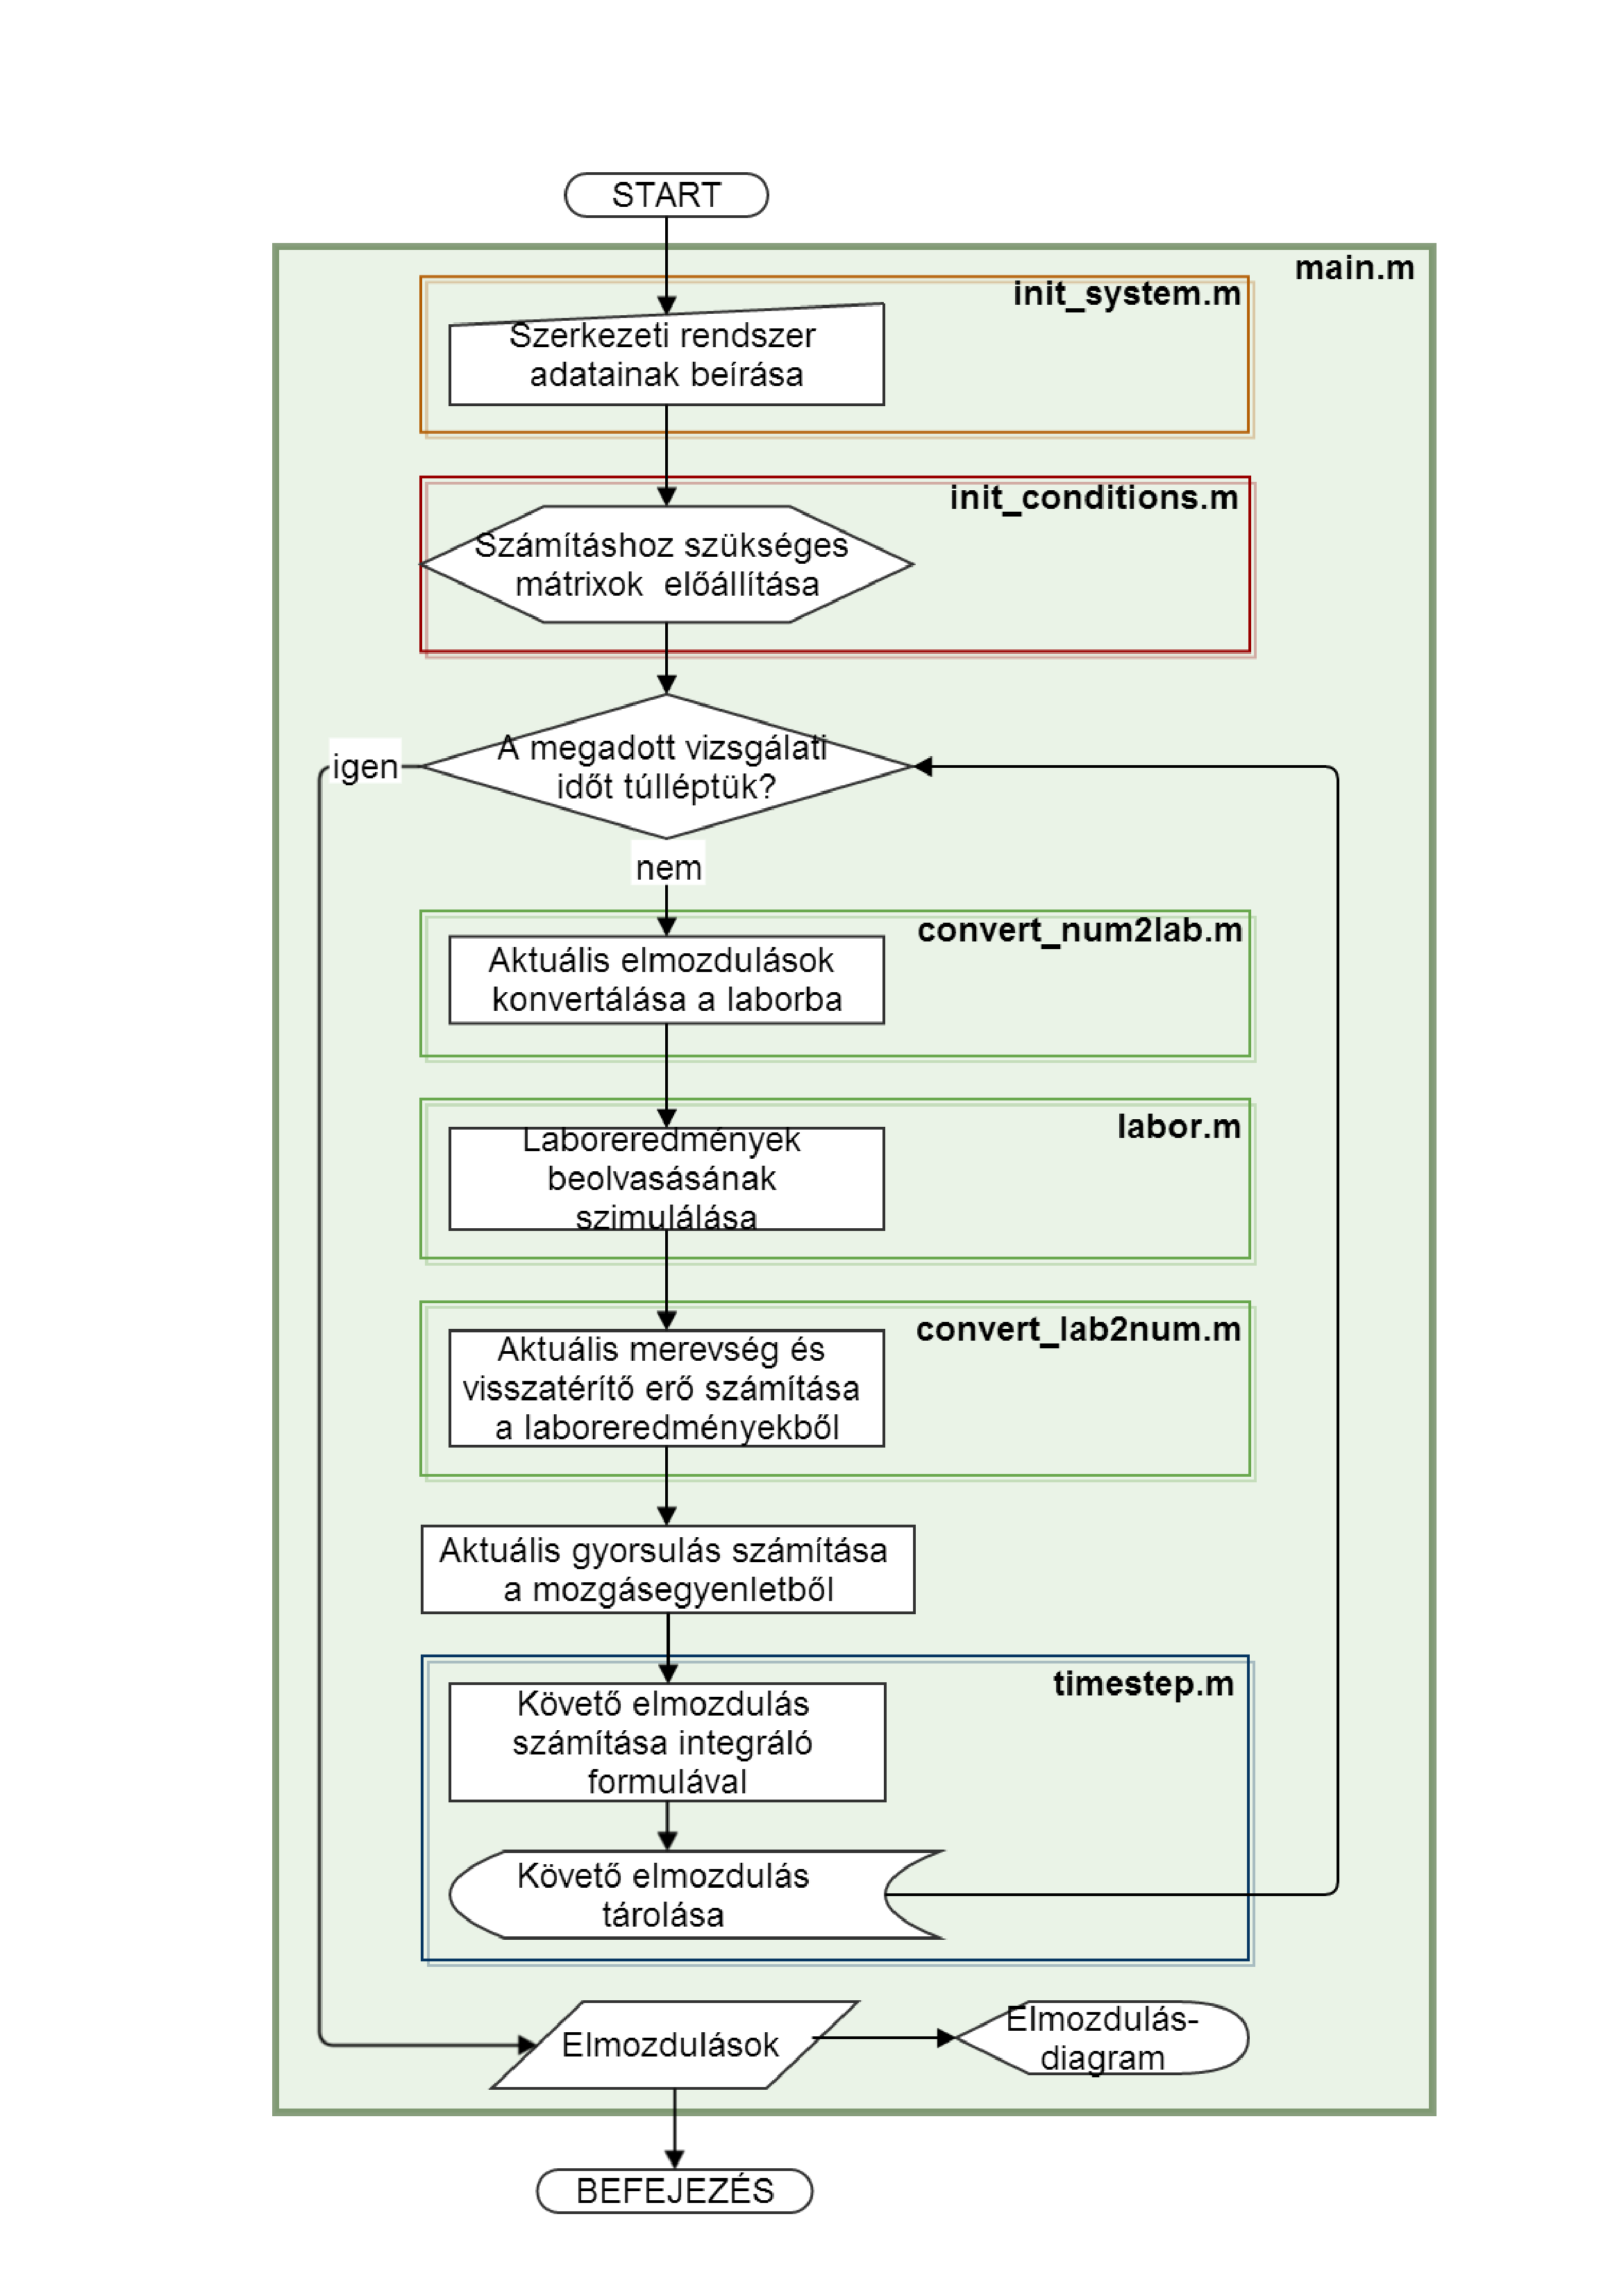
\includegraphics[trim = 0mm 5mm 0mm 40mm, clip, width=\textwidth]{hibrid_folyamatabra.pdf}
\caption{A hibrid program folyamatábrája.}
\label{fig:hibridprog_folyamatabra}
\end{figure}

A program műveleti blokkokból áll. Ezek egy része összeegyeztethető a lineáris és nemlineáris megoldóknál használtakkal. A \verb|main.m| szkript a műveleti parancssort és a beillesztett műveleti blokkokat tartalmazza. Az első lépés egy biztonsági törlés elvégzése. Ezt követően a szkript meghívja az \verb|init_system.m| fájlt, és beolvassa a vizsgált szerkezet alapadatait, majd az \verb|init_conditions.m| szkriptet hívja, ami a számítás előkészületeként a helyfoglaló és a  segédmátrixokat állítja elő. Ezt követi a kísérleti vizsgálatot és a numerikus számítást végző for ciklus. A ciklusban a \verb|convert_num2lab.m| végzi a kezdeti értékek és a numerikus számításokból adódó értékek konvertálását, a \verb|labor.m| szkript szimulálja a laboratóriumi kísérletet , a laboratóriumi kísérletekből kapott eredményeket pedig a \verb|covert_lab2num.m| fájl konvertálja a numerikus számításhoz. Ekkor az aktuális  időlépéshez tartozó gyorsulás számítása következik, majd a \verb|timestep.m| szkript elvégzi a numerikus integrálást, és elmenti az eredményül kapott, a következő időlépéshez tartozó elmozdulást. A for ciklus futása az előre megadott vizsgálati időintervallum végéig tart. Az utolsó lépés az eredmény kirajzolása egy elmozdulás - idő diagramban.

Az \verb|init_system.m| szkriptben a vizsgálat  adatait és a kezdeti feltételeket adhatjuk meg. Ezek  a vizsgálat időtartama, az időlépések nagysága, a szerkezet tömeg-, a merevségi és csillapítási mátrixa, a tehervektor, valamint a $\mathbf{u}_0$ és  $\mathbf{\dot{u}}_0$  kezdeti feltételek. Itt kell megadnunk továbbá, hogy a kísérleti próbatesten a terhelést hány lépcsőben végezzük. Ha az adott feladatban szükséges, számítjuk a szerkezet sajátkörfrekvenciáit és sajátrezgésalakjait. A csillapítási mátrix számítása is ebben a szkriptben történik. A csillapítási mátrixhoz alapvetően arányos csillapítást vesz figyelembe a program, de ezt lehet módosítani, ha a feladat megkívánja. A kezdeti feltételeken túl esetenként meg kell adni az első lépésben a labornak a  szükséges értékeket, mint a kezdeti visszatérítő erő és érintőmerevség, valamint a próbatestre alkalmazandó kezdeti elmozdulás.

Az \verb|init_conditions.m| szkript lefoglalja a helyet az elmozdulásvektoroknak, és elvégzi a számítás alatt állandó segédmátrixok előállítását és invertálását, ha szükséges. 

A \verb|convert_num2lab.m| fájl konvertálja a kezdeti feltételekből vagy a numerikus számításokból ismert aktuális elmozdulást. A program a laborban történő alkalmazáshoz szükséges geometriai összefüggéseket is itt számolja. Ehhez az \verb|U_num2lab.m| függvényt hívja meg, ami átszámolja a szerkezet globális koordináta-rendszeréből a próbatest lokális koordináta-rendszerébe az aktuális elmozdulást.

A \verb|labor.m| szkript a laborkísérletet szimulálja. Szükség esetén ezt viszonylag egyszerűen kiválthatja  a tényleges laboratóriumi vizsgálat. A  kísérletben először tároljuk az előző lépésben mért visszatérítő erőt. Az aktuális elmozdulást az \verb|init_system.m| fájlban megadott számú lépcsőben érjük el. Az utolsó előtti szakaszban mérjük az elmozduláslépcsőhöz tartozó visszatérítő erőt, majd ennek segítségével extrapolálunk az utolsó elmozduláslépcsőhöz tartozó értékre. Az elmozdulás és a visszatérítő erő változásából ekkor számíthatjuk az aktuális érintőmerevséget. A szimulált laborkísérlet annyiban különbözik a valóstól, hogy a visszatérítő erő  értékét nem mérjük, hanem számítjuk. Ehhez a \verb|resisting_force.m| függvényt hívjuk, ami a feltételezett anyagmodell alapján számítja a visszatérítő erő értékét. 

Ezt követően a laboreredményeket, az aktuális visszatérítő erőt és a próbatest aktuális érintőmerevséget konvertáljuk a numerikus számításhoz a \verb|covert_lab2num.m| szkriptben. Ekkor a próbatest lokális koordináta-rendszeréből át kell számolnunk az eredményeket a szerkezet globális koordináta-rendszerébe. Ehhez az \verb|f_s_lab2num.m| függvényt használjuk. Ha ez megtörtént, számítjuk a szerkezet aktuális merevségi mátrixát. 

A laborból konvertált adatokkal már számítható a mozgásegyenletből  az aktuális gyorsulásvektor. A \verb|timestep.m| fájl a CR algoritmus időlépéséhez tartozó lépésekkel  explicit módon számítja és tárolja a következő időponthoz tartozó elmozdulást és sebességet. Hibrid módszernél, mivel a merevségi mátrix nem állandó, az $\boldsymbol\alpha_1$
 és  $\boldsymbol\alpha_1$ integráló paramétereket is lépésenként kell számítani. 


\section{A program használatának bemutatása}\label{sec:hibr_példa}

{\ }

A hibrid szimulációs program műveleti blokkokból áll, így az egyes feladatokhoz elég néhány blokkot módosítani. Ezek általános esetben a bemeneti adatokat tartalmazó \verb|init_system.m|, valamint a globális és lokális koordináta-rendszerek közötti összefüggést meghatározó \verb|U_num2lab.m| és  \verb|f_s_lab2num.m| fájlok.  A vizsgált szerkezet paramétereit, a merevségi és tömegmátrixokat, a csillapítási mátrix előállatásának módját, a szerkezetre ható terhelést és a kezdeti feltételeket, illetve a labornak küldött kezdeti értékeket mind az \verb|init_system.m| szkriptben módosíthatjuk. A szerkezet geometriája alapján a globális koordináta-rendszer és a próbatest lokális koordináta-rendszere közötti átszámítás képleteit  az \verb|U_num2lab.m| és az \verb|f_s_lab2num.m| függvényekben adhatjuk meg. 

Szimulált hibrid szimuláció esetében megválaszthatjuk továbbá, hogy milyen anyagmodellt veszünk figyelembe a nemlineáris viselkedésű próbatestnél.  Az anyagmodell számítását a \verb|resisting_force.m| függvényben adhatjuk meg, mivel annak változása  a visszatérítő erőben jelenik meg.

A szimulált kísérletről a valós kísérleti eljárásra való áttéréshez a \verb|labor.m| szkriptben számított aktuális visszatérítő erő és érintőmerevség helyett  a laboratóriumi kísérletben mért értékeket használjuk. Ehhez a \verb|labor.m| fájlt ki kell cserélni egy olyan  szkriptre, ami ezeket az értékeket beolvassa.

\begin{figure}[h!]
\centering
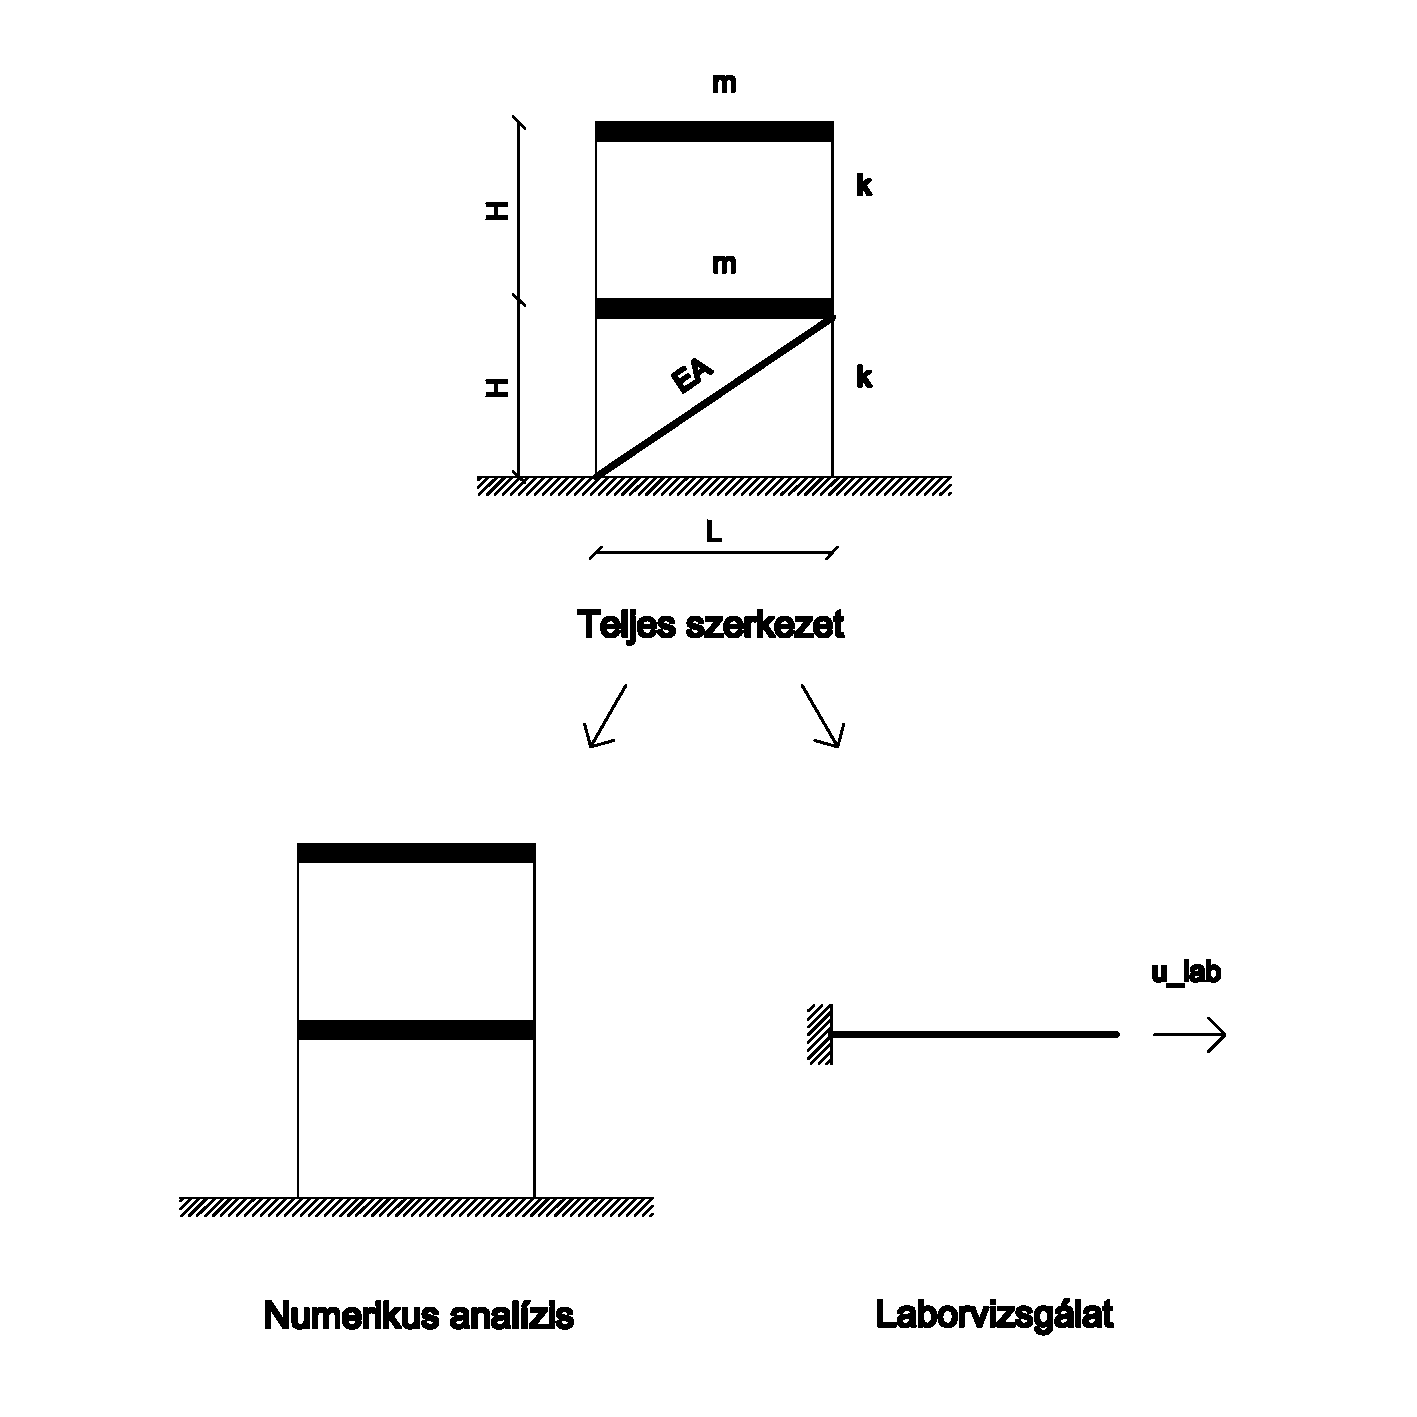
\includegraphics[ width=0.8\textwidth]{hidrid_abra.pdf}
\caption{A hibrid szimulációs programmal vizsgált szerkezet  és szétbontása.}
\label{fig:hibridprogpélda}
\end{figure}


A program használatát egy konkrét példán mutatom be. Adott a \ref{fig:hibridprogpélda} ábrán látható kétszintes keret, az alsó szinten egy ferde, nemlineáris viselkedésű merevítő rúddal. A rendszer modellezését a \ref{fig:viselkedési modell} ábrán láthatjuk. A feladatban a merevítő rúd viselkedését  szimulált laborkísérlettel, a  szerkezet többi részét pedig numerikusan vizsgáljuk. A szerkezet fesztávolsága és a szintek magassága egyaránt $3 m$. Az egyes szintek tömege $m = 45 t$, a szintenkénti merevség $k = 18000 kN/m$. A merevítő rúd merevsége $EA = 76367 kN$.  Modellezésére a \ref{subsec:nemlinstat} pontban a nemlineáris programnál bemutatott nemlineárisan rugalmas anyagmodellt használjuk, és a rúd megnyúlását pontosan számítjuk. Ezzel egy geometriai és egy anyagi nemlinearitást is figyelembe veszünk. A  szerkezeten arányos csillapítást alkalmazunk, $\alpha$ és $\beta$ értékét úgy vesszük fel, hogy mindkét módban $\xi$ tényező értéke $5\%$ legyen.   A kezdeti feltételek,  a laborvizsgálathoz szükséges  kezdeti visszatérítő erő és érintőmerevség, valamint a próbaestre alkalmazandó kezdeti elmozdulás értéke zérus.

\begin{figure}[h!]
\centering
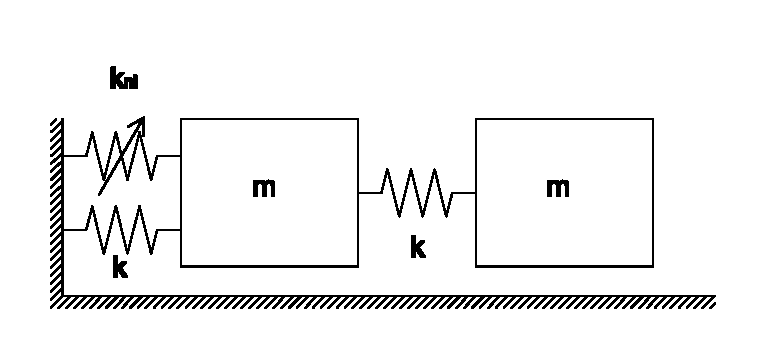
\includegraphics[ width=0.6\textwidth]{nemlin_modell.pdf}
\caption{A hibrid szimulációs programmal vizsgált szerkezet modellezése.}
\label{fig:viselkedési modell}
\end{figure}

A szerkezetet adatai képletekkel:
\begin{align*}
  & L = 3 m  & & H = 3 m   & \\
  & EA = 76367 kN & k_n = \frac{EA}{\sqrt{L^2+H^2}} & \\
  & \mathbf{M}  = \left[\begin{array}{rr}  45 & 0 \\ 0 & 45 \end{array} \right]t   &  & \mathbf{K} = 18000\left[\begin{array}{rr} 2 & -1 \\ -1 & 1 \end{array} \right]\frac{kN}{m}  &  \\
  & \mathbf{C}  = \alpha\mathbf{M}+\beta\mathbf{K}  &  & \xi = 0,05  & \\
  & \mathbf{u}(0)  = \left[\begin{array}{c} 0 \\ 0 \end{array} \right]  & & \mathbf{\dot{u}}(0) = \left[\begin{array}{c} 0 \\ 0 \end{array} \right] & \\
  & f_{s,lab,0} = 0 kN & &U_{lab,0} = 0 m   & \\
  & k_{t,lab,0} = k_n  & & f_s(\Delta{l})  = a \arctan{b\Delta{l}}&
  \end{align*}

Ezek alapján  az \verb|init_system.m| fájl a következő:

 \lstinputlisting{"MATLAB/hibrid/init_system.m"}
 
 
 A szerkezet geometrája alapján a globális és lokális koordináta-rendszerek közötti átszámítást leíró \verb|U_num2lab.m| és \verb|f_s_lab2num.m| függvények:
 
 \lstinputlisting{"MATLAB/hibrid/U_num2lab.m"}
 \lstinputlisting{"MATLAB/hibrid/f_s_lab2num.m"}


 A  \verb|resisting_force.m| függvény a szerkezet anyagmodellje alapján a következő:
 
  \lstinputlisting{"MATLAB/hibrid/resisting_force.m"}
 
  
  A példán keresztül látható, hogy a szerkezet bemeneti adatainak megadására szolgáló fájlok elkülönülnek a számítást végző műveleti blokkoktól, így a program módosítása az egyes feladatokhoz viszonylag egyszerűen elvégezhető. 
  
  
\section{Hibrid szimulációs program verifikálása}\label{sec: hibrid ver.}

{\ }

A következőkben a hibrid szimulációs program verifikálását végzem el a \ref{sec:hibr_példa} alfejezetben bemutatott kétszintes merevített kereten. A vizsgálati eredményeket ugyanazon a szerkezeten végzett nemlineáris számítás eredményeivel hasonlítom össze.


\subsection{Kijelölt szerkezet vizsgálata hibrid szimulációval}\label{subsec:71_hibrid}

{\ }

A szerkezetre teherként az El Centro földrengés gyorsulásaiból számított földrengésterhet működtetem.  A földrengés a valóságban már lezajlott 1940-ben  Kalifornia államban. Az El Centro-t gyakran alkalmazzák a földrengésszámítások során.  A \ref{fig:ec gyors}  ábrán az El Centro földrengés gyorsulásai  láthatók az idő függvényében. Az adatok a Vibrationdata  \cite{elcentro} honlapjáról származnak.

\begin{figure}[h!]
\centering
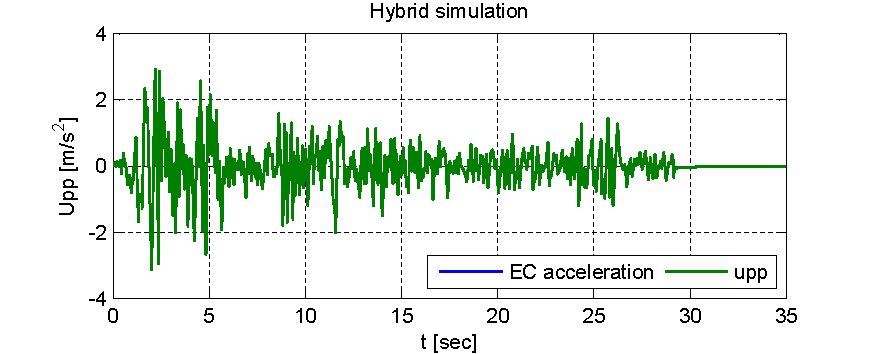
\includegraphics[width=\textwidth]{72_gyorulas_EC.pdf}
\caption{Az El Centro földrengés gyorsulásai.}
\label{fig:ec gyors}
\end{figure}

Az El Centro gyorsulásadatait  a programba az \verb|EQ_load.m| függvénnyel töltöm be. A függvény a  gyorsulásadatok beolvasását  és a vizsgált diszkrét időpontbeli értékek interpolálását végzi el.  A függvény a Függelék \ref{chap: függ hibrid prog}. pontjában látható. 

A tehervektor számítása a gyorsulásokból a \eqref{támrezg1} támaszrezgés  egyenletéből adódik:

\begin{equation}
 \mathbf{q} = -\mathbf{M}\mathbf{\ddot{u}}_g(t)
\end{equation} 

Az \verb|init_system.m| fájlban a tehervektor megadása  a következőképpen alakul:
 \lstinputlisting[firstline=53, lastline=66]{"MATLAB/hibrid_72/init_system.m"}
 
A szimulációból kapott elmozdulásokat az idő függvényében a \ref{fig:ec_elm-a} ábrán láthatjuk.


\subsection{Kijelölt szerkezet vizsgálata nemlineáris analízissel}

{\ }

A nemlineáris programban ugyanazt a \ref{fig:hibridprogpélda} ábrán látható kétszintes keretet számoltuk. Az elmozdulásokat a Newmark módszer elmozdulásos változatával számoltuk. A szerkezetre a nemlineáris programban is az El Centro-t működtetem. A gyorsulásadatok betöltését ugyanúgy az \verb|EQ_load.m| függvénnyel végeztem. Az \verb|init_system.m| szkriptben csak a kezdeti feltételek megadása különbözik a hibrid szimulációnál látottaktól:

 \lstinputlisting[firstline=69, lastline=84]{"MATLAB/nonlinear_system_71/init_system.m"}

A nemlineáris merevítő rúd  anyagmodellje megegyezik a hibrid számításnál alkalmazottal, így ugyanazt a geometriai és anyagi nemlinearitást vesszük figyelembe. Ez alapján programban a visszatérítő erő számítása a \verb|resisting_force.m| és az érintőmerevségé a \verb|tangent_stiffness.m| függvényekben a következő:

\lstinputlisting{"MATLAB/nonlinear_system_71/resisting_force.m"}
\lstinputlisting{"MATLAB/nonlinear_system_71/tangent_stiffness.m"}


\subsection{A nemlineáris és a hibrid szimulációs program eredményeinek összehasonlítása}

{\ }

A feladat hibrid és nemlineáris számításából a \ref{fig:ec_elm-a} és \ref{fig:ec_elm-b} ábrákat összehasonlítva szemre hasonló eredményeket kaptunk. A két ábra között igazán nincs  különbség,  ha egymás fölé vetítjük ezeket, akkor is csak minimális  eltérés figyelhető meg. 

\begin{figure}[h!]%
\centering
\subfigure[][]{%
\label{fig:ec_elm-a}%
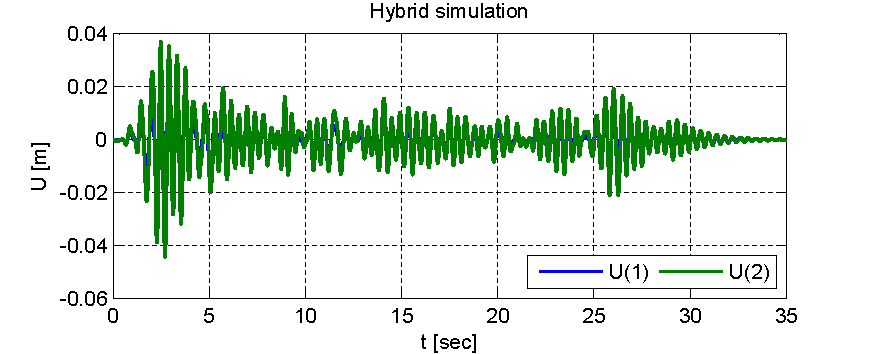
\includegraphics[width=\textwidth]{72_elmozdulas.pdf}}%
\\
\subfigure[][]{%
\label{fig:ec_elm-b}%
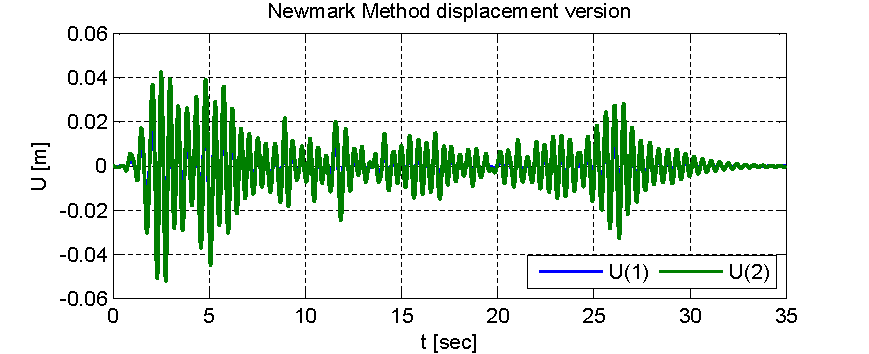
\includegraphics[width=\textwidth]{71_elmozdulas.pdf}}%
\caption[Kétszintes merevített keret elmozdulásai.]{Kétszintes merevített keret elmozdulásai az El Centro földrengés hatására:
\subref{fig:ec_elm-a} hibrid szimulációval;
\subref{fig:ec_elm-b} nemlineáris számítással.}%
\label{fig:ec_elm}%
\end{figure}

Azonban méretezési feladatokban  nem annyira az időbeni lefutás fontos, hanem az eredmények  maximum (abszolút)értékei, ezért kiválogattam ezeket, és összegyűjtöttem a \ref{7_table} táblázatba. Fontos megjegyezni, hogy ezek tényleges értékek, nem pedig a modálanalízis egyes eredményeinek valamilyen közelítésen alapuló összegzése. 
A táblázatból látszik, hogy a számítások között minimális a különbség. A maximális elmozdulások között az eltérés nagyságrendileg néhány milliméter.

\begin{table}[h!]
\centering
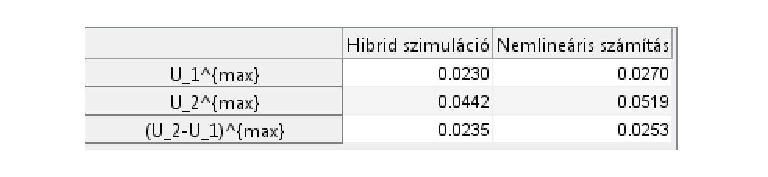
\includegraphics[width=0.7\textwidth]{7_table.pdf}
\caption{A hibrid és a nemlineáris programmal számított maximális elmozdulások.}
\label{7_table}
\end{table}
